\vspace{2cm}
\rhead{SENSITIVITY ANALYSIS}
\chapter{Introduction}
\lhead{Introduction}
Sensitivity analysis (SA) studies how changes in the input of a model affect the output, and it is essential for many engineering applications, such as uncertainty quantification, optimal design, and to answer \textit{what if} questions, i.e. what happens to the solution of the model if the input parameters change. These tasks can be performed in many different ways, depending on the nature of the model considered. In this work, we consider systems that can be modelled with partial differential equations (PDEs). The sensitivity variable itself is defined as the derivative of the state (i.e., the output of the model) with respect to the parameters of interest. 

In the framework of PDEs, one can distinguish two main classes of methods: the \textit{differentiate-then-discretise} methods and the \textit{discretise-then-differentiate} methods. As the names say, in the first case the state model is formally differentiated with respect to the parameter of interest, providing an analytical sensitivity system which can then be discretised with the most appropriate numerical scheme. The second class of methods swaps the two steps which, in the general case, are not commutative. A detailed comparison between the two classes of methods can be found in \cite{gunzburger2003perspectives} for optimisation problems. 
In this work, we focus on the first class, and, in particular, on the continuous sensitivity equation method \cite{Borggaard1997366,duvigneau2006improved,Duvigneau_Pelletier_06_ijcfd,chalons2018sensitivity, SA_Euler}.

The main aim of this work is to give an estimate of the variance of the solution of the Navier--Stokes equations when there are uncertain parameters and then to use the estimated variance to compute confidence intervals. This goes under the name of forward uncertainty propagation, which is part of the broader field of uncertainty quantification (UQ). Many strategies and techniques have been proposed in the literature to tackle UQ problems, particularly in the case of PDEs models: Monte Carlo method \cite{christian1999monte}, polynomial chaos \cite{Walters_03, Xiu_et_Karniadakis_03, Knio_LeMaitre_06, Despres2013}, random space partition \cite{abgrall_congedo_13}, to name but a few. A review of these methods applied to fluid dynamics problems can be found in \cite{walters2002uncertainty}. 

Methods of uncertainty propagation based on SA are particularly efficient in terms of computational time if compared, for instance, to methods like Monte Carlo. However, since SA is based on Taylor expansions of the state variable with respect to the parameter of interest, these methods are intrinsically local \cite{delenne2014propagation}~: they can be used only for random variables with a small variance. The Monte Carlo approach does not require this assumption; however, it is not applicable for realistic unsteady test cases in $2D$ and $3D$, due to its high computational cost. In this work we propose an approach based on the sensitivity equation method: under the hypothesis of small variance of the input parameters, we can provide a first-order estimate of the variance of the solution at a reasonable computational cost. 
\newpage
\rhead{SENSITIVITY ANALYSIS}
\chapter{The physical model}
\lhead{The physical model}
\label{sec_physical_model}
In this section, we present the physical model as well as some stability estimates for it and its sensitivity.
\section{The state equations}
Let us consider the domain $\Omega$ in Figure~\ref{domain}: it is a channel with walls on the top and the bottom and an obstacle of square section at distance $x_D$ from the inflow boundary. The Navier-Stokes system and the boundary conditions for this domain are:
\begin{figure}[h]
\begin{center}
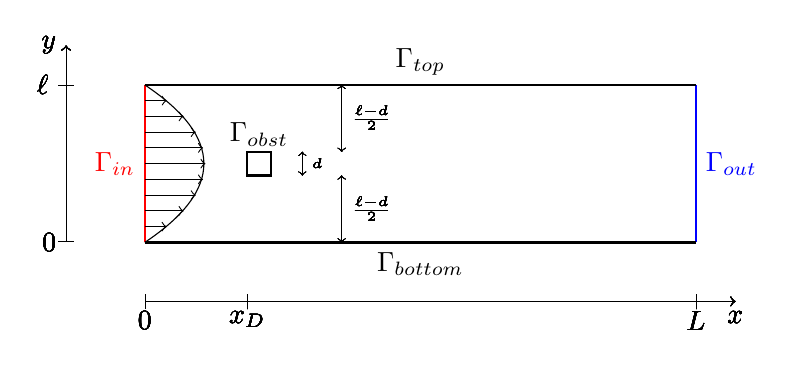
\begin{tikzpicture}
\draw[thick, red] (0,0) -- (0,2);
\draw[thick, blue] (7,0) -- (7,2);
\draw[thick] (1.3,0.85) rectangle (1.6,1.15);
\draw[thick] (0,0) -- (7,0);
\draw[thick] (0,2) -- (7,2);
\node[left] at (0,1) {\color{red}$\Gamma_{in}$};
\node[right] at (7,1) {\color{blue}$\Gamma_{out}$};
\node[above] at (3.5,2) {$\Gamma_{top}$};
\node[below] at (3.5,0) {$\Gamma_{bottom}$};
\node[above] at (1.45,1.1) {$\Gamma_{obst}$};
\draw[thin] (0,0) .. controls (1,2/3) and (1, 4/3) .. (0,2);
\foreach \y in {2, 4, ..., 18}{
\draw[thin,->] (0,0.1*\y) -- (0.2*\y*0.77-0.01*\y*\y*0.77,0.1*\y);
%asse y
\draw[thin,|->] (-1,0)--(-1,2.5);
\draw[very thin] (-1.1,2)--(-0.9,2);
\node[left] at (-1,0) {$0$};
\node[left] at (-1.1,2) {$\ell$};
\node[left] at (-1,2.5) {$y$};
%asse x
\draw[thin,|->] (0,-.75)--(7.5,-.75);
\draw[very thin] (1.3,-.85)--(1.3,-0.65);
\draw[very thin] (7,-.85)--(7,-0.65);
\node[below] at (0,-.75) {$0$};
\node[below] at (1.3,-.75) {$x_D$};
\node[below] at (7,-.75) {$L$};
\node[below] at (7.5,-.75) {$x$};
%misura e posizione ostacolo
\draw[very thin, <->] (2, 0.85)--(2, 1.15);
\node[right] at (2,1) {\tiny $d$};
\draw[very thin, <->] (2.5, 0)--(2.5, 0.85 );
\node[right] at (2.5,0.425) {\tiny $\frac{\ell-d}{2}$};
\draw[very thin, <->] (2.5, 1.15)--(2.5, 2);
\node[right] at (2.5,1.575) {\tiny $\frac{\ell-d}{2}$};
}
\end{tikzpicture}
\caption{Domain for the first test case.}
\label{domain}
\end{center}
\end{figure}

\begin{equation}
\begin{cases}
\partial_t \b_u - \nu \Delta \b_u + (\b_u \cdot \nabla) \b_u + \nabla p = \mathbf{f}& \Omega, t > 0, \\
\nabla \cdot \b_u = 0 & \Omega, t>0, \\
\b_u (\mathbf{x}, 0) = 0 & \Omega, t=0, \\
\b_u = - g(y)\mathbf{n} & \text{on } \Gamma_{in}, \\
\b_u = 0 & \text{on } \Gamma_w = \Gamma_{obst} \cup \Gamma_{top} \cup \Gamma_{bottom}, \\
(\nu \nabla \b_u -pI) \mathbf{n} = 0 & \text{on } \Gamma_{out},
\end{cases}
\label{state}
\end{equation}
where $\b_u = (u^x, u^y)^t$ is the velocity, $p$ is the pressure, $\mathbf{f}$ the external force and $g(y)$ the prescribed inflow condition. The first equation models the conservation of the momentum and the second one the conservation of the mass. In the following, they will be referred to as, respectively, the momentum equation and the mass equation. We impose no slip boundary condition of the walls of the domain, a prescribed velocity at the inflow and a homogeneous Neumann boundary condition at the outflow. 


\section{The sensitivity equations}
We now consider $\b_u$ as a function of space, time and a scalar uncertain parameter $a$, $\b_u = \b_u(\mathbf{x},t;a)$ and we write a formal Taylor expansion with respect to $a$:
\begin{equation}
\b_u(\mathbf{x},t;a+\delta a) = \displaystyle \sum_{k=0}^\infty \b_u_k(\mathbf{x},t;a) \delta a^k,
\label{series}
\end{equation}
where $\b_u_0 = \b_u$ and the coefficient $\b_u_k$ is the $k-$th derivative of $\b_u$ with respect to $a$:
\[
\b_u_k(\mathbf{x},t;a) := \frac{d^k}{da^k} \b_u(\mathbf{x},t;a),
\]
and it is called the $k-$th order sensitivity. To consider more than one parameter of interest, the sensitivity should be defined as the gradient of the state with respect to the vector of parameters and a multi-dimensional Taylor expansion would be necessary, but this is not treated in this work. A similar expansion can be done for the pressure $p$, and the data $\mathbf{f}$, $\mathbf{d}$, and $g$. In order to write the equations for the sensitivities, one can replace (\ref{series}) into (\ref{state}) and then factorise according to the powers of $\delta a$. For $k=0$ we obtain the state system (\ref{state}). For $k=1$, we obtain the first order sensitivity equations. In this work, we consider only first-order sensitivity and the notation $\b_u_1 = \b_u_a$ will be employed. This choice is common \cite{Borggaard1997366, duvigneau2006improved, Duvigneau_Pelletier_06_ijcfd, chalons2018sensitivity, SA_Euler} because in most cases first order sensitivities provide enough information. It is possible to consider higher order sensitivities if necessary, but this is not investigated in this work. The first order sensitivity equations, referred to as the sensitivity equations in short, are:
\begin{equation}
\begin{cases}
\partial_t \b_u_a - \nu \Delta \b_u_a + (\b_u_a \cdot \nabla) \b_u + (\b_u \cdot \nabla) \b_u_a + \nabla p_a = \mathbf{f}_a& \Omega, t > 0, \\
\nabla \cdot \b_u_a = 0 & \Omega, t>0, \\
\b_u_a (\mathbf{x}, 0) = 0 & \Omega, t=0, \\
\b_u_a = - g_a(y)\mathbf{n} & \text{on } \Gamma_{in}, \\
\b_u_a = 0 & \text{on } \Gamma_w , \\
(\nu \nabla \b_u_a -p_aI) \mathbf{n} = 0 & \text{on } \Gamma_{out},
\end{cases}
\label{sensitivity}
\end{equation}
where $\Gamma_w := \Gamma_{obst} \cup \Gamma_{top} \cup \Gamma_{bottom}$.
These are known as the Oseen equations: an introduction on the subject can be found in \cite{john2014oseen}, both for the theoretical and the numerical aspects. A similar problem is investigated, although only from a numerical point of view, in \cite{duvigneau2005evaluation,duvigneau2006improved}, where they use the sensitivity for shape optimization problems: in their case an expansion of the normal $\mathbf{n} = \sum \mathbf{n}_k(\mathbf{x};a)\delta a^k$ is necessary, which leads to more complicated boundary conditions.
Remark: if $\nu$ is considered as the parameter of interest, the second member of the first equation should be $\overline{\mathbf{f}}_a := \mathbf{f}_a+\nu_a\Delta\b_u$ and the Neumann boundary condition should have the additional term $\nu_a\nabla\b_u\ \mathbf{n}$, but this case is not considered in this work. 

\rhead{SENSITIVITY ANALYSIS}
\chapter{Uncertainty propagation}
\lhead{Uncertainty propagation}
\label{sec_uq}
In this section, we want to show how the sensitivity can be used to give a first order estimate of the variance of the model output. In this context, the parameter $a$ is a random variable with a known distribution, expected value $\mu_a$, and variance $\sigma_a^2$. Let $X(\mathbf{x},t;a)$ be a physical variable (i.e. the horizontal or vertical velocity, or the pressure), whose expected value $\mu_X$ and variance $\sigma_X^2$ we want to estimate. To do this, we start from a Taylor expansion of $X$ with respect to the parameter  $a$ centred in the expected value of $a$, $\mu_a$:
\begin{equation}
X(\mathbf{x},t;a) = X(\mathbf{x},t;\mu_a) + (a-\mu_a)X_a(\mathbf{x},t;a) + o(|a-\mu_a|^2),
\label{taylor_exp}
\end{equation}
where $X_a = \partial_a X$ is the sensitivity of $X$ with respect to the parameter $a$. Computing the expected value of the right and left-hand side of (\ref{taylor_exp}), one obtains the following first order estimate:
\begin{equation}
\mu_X(\mathbf{x},t) = E[X(\mathbf{x},t;a)] \simeq X(\mathbf{x},t;\mu_a) + E[(a-\mu_a)]X_a(\mathbf{x},t;a) = X(\mathbf{x},t;\mu_a).
\label{average}
\end{equation}
Using again the Taylor expansion (\ref{taylor_exp}) and the estimate just obtained for the average (\ref{average}), we obtain an estimate of the variance:
\begin{equation}
\sigma_X^2(\mathbf{x},t) = E[(X(\mathbf{x},t;a)-\mu_X(\mathbf{x},t))^2] \simeq E[(a-\mu_a)^2]X_a^2(\mathbf{x},t;a) = \sigma_a^2 X_a^2(\mathbf{x},t;a).
\label{variance}
\end{equation}
The estimates (\ref{average})-(\ref{variance}) are valid only where the Taylor expansion (\ref{taylor_exp}) holds, i.e. for small variances of the random parameter $\sigma_a^2$. However, one can have an estimate of the variance with just one simulation of the state and one of the sensitivity, which is a minimal computational cost when compared to methods such as Monte Carlo that require thousands of simulations of the state to estimate the variance. In the general case, when more than one parameter is uncertain, to provide an estimate of the variance, one would need one simulation for the state and as many simulations of the sensitivity as the number of uncertain parameters \cite{fiorini2018phd}. This makes the sensitivity approach really affordable and highly competitive when the number of uncertain parameters is small enough. In the next subsection, we compare the results of the SA approach with the well-known Monte Carlo method \cite{christian1999monte}.

The estimated variance can be used for multiple purposes. In this work, we use it to compute some confidence intervals for the physical variables, i.e. find an interval $CI_X$ such that the probability that $X$ falls into $CI_X$ is bigger that $1-\alpha$. Standard choices for $\alpha$ are $0.05$ or $0.01$. If the distribution of the random variable $X$ is known, some precise estimates for the extrema of the interval exist. However, SA does not provide any insight of what the distribution of the output is. Therefore we start from Chebyshev inequality \cite{jacod2012probability}, which states that for any random variable with finite expected value and variance
\[
P(|X-\mu_X| \geq \lambda) \leq \frac{\sigma^2_X}{\lambda^2}.
\]
By imposing the desired level for confidence interval, i.e. $\alpha = \frac{\sigma^2_X}{\lambda^2}$, one gets $\lambda = \frac{\sigma_X}{\sqrt{\alpha}}$, therefore
\begin{equation}
CI_X = \left[\mu_X - \frac{\sigma_X}{\sqrt{\alpha}}, \mu_X + \frac{\sigma_X}{\sqrt{\alpha}}\right].
\label{CI}
\end{equation}



%\bibliographystyle{alpha}

